\documentclass[border=10pt]{standalone}

\usepackage{tikz}
\usepackage{tikzsymbols}
\usetikzlibrary{calc,patterns,shapes.geometric}

\def\centerarc[#1](#2)(#3:#4:#5){\draw[#1] ($(#2)+({#5*cos(#3)},{#5*sin(#3)})$) arc (#3:#4:#5);}

\begin{document}
	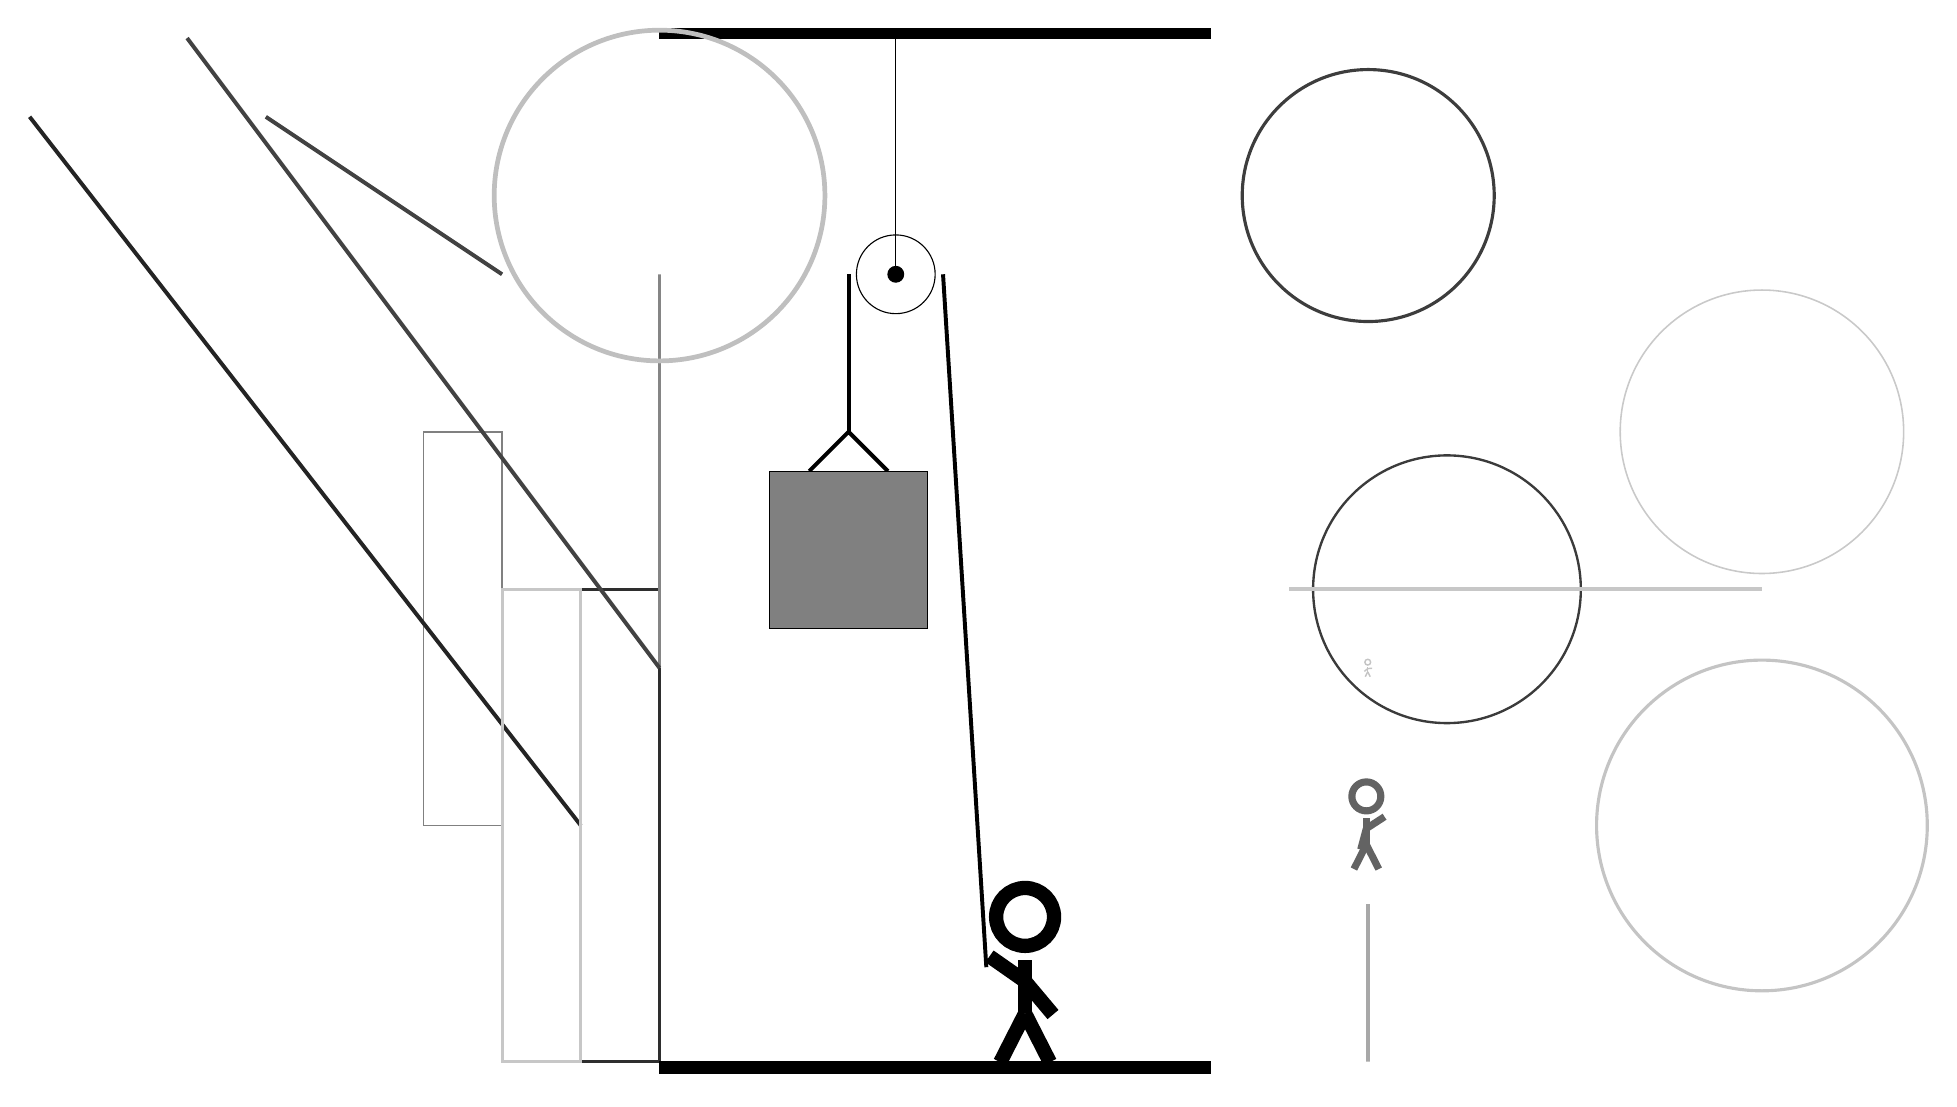
\begin{tikzpicture}
		%%%%% START %%%%%
		
		\draw[fill=black] (-2, 10) rectangle (5, 10.125);
		
		\draw (1, 7) circle (0.5);
		\draw[fill=black] (1, 7) circle (0.1);
		\draw (1, 10) -- (1, 7);
		
		\draw[line width=0.5mm] (-0.1, 4.5) -- (0.4, 5.0) -- (0.9, 4.5);
		\draw[fill=black!50] (-0.6, 4.5) rectangle (1.4, 2.5);
		
		\draw[line width=0.5mm] (0.4, 7) -- (0.4, 5.0);
		\centerarc[line width=0.5mm](1, 7)(0:180:0.6);
		\draw[line width=0.5mm](1.6, 7) -- (2.15, -1.8);
		
		\draw [line width=0.2mm, color=black!21](12, 5) circle (1.8);
		
		\draw[line width=0.5mm, color=black!74](-7, 9) -- (-4, 7);
		\draw[line width=0.2mm, color=black!50] (-4, 5) rectangle (-5, 0);
		\draw[line width=0.4mm, color=black!82] (-2, -3) rectangle (-3, 3);
		
		\node[line width=0.6mm, color=black!61] at (7, 0) {\Strichmaxerl[5][75][33]};
		
		\draw [line width=0.4mm, color=black!76](7, 8) circle (1.6);
		
		\draw [line width=0.3mm, color=black!77](8, 3) circle (1.7);
		\draw[line width=0.4mm, color=black!48] (-2, 2) rectangle (-2, 7);
		\draw[line width=0.5mm, color=black!86](-3, 0) -- (-10, 9);
		
		\node[line width=0.3mm, color=black!23] at (7, 2) {\Strichmaxerl[1][39][5]};
		\draw [line width=0.4mm, color=black!23](12, 0) circle (2.1);
		\draw[line width=0.5mm, color=black!22](6, 3) -- (12, 3);
		\draw [line width=0.6mm, color=black!25](-2, 8) circle (2.1);
		\draw[line width=0.4mm, color=black!22] (-3, -3) rectangle (-4, 3);
		\draw[line width=0.5mm, color=black!34] (7, -3) rectangle (7, -1);
		\draw[line width=0.5mm, color=black!74](-2, 2) -- (-8, 10);
		
		
		\node at (2.6, -1.9) {\Strichmaxerl[10][-35][-50]};
		
		\draw[fill=black] (-2, -3) rectangle (5, -3.15);
		
		%%%%% END %%%%%
	\end{tikzpicture}
\end{document}